\documentclass[12pt, letterpaper]{report}

%---------PACKAGES-------------
\usepackage[utf8]{inputenc}
\usepackage[T1]{fontenc}
\usepackage[margin=1in]{geometry}
%\usepackage{1modern}
\usepackage{setspace}
\usepackage{graphicx}
\usepackage{float}
\usepackage{caption}
\usepackage{booktabs}
\usepackage{amsmath, amssymb}
%\usepackage{sinuitx}
\usepackage{hyperref}
\usepackage{fancyhdr}
\usepackage{lineno}
\usepackage{tocloft}
\usepackage{titlesec}
\usepackage{xcolor}
\usepackage{listings}

%----------HYPERREF-----------
\hypersetup{
    colorlinks=true,
    linkcolor=blue,
    citecolor=blue,
    urlcolor=blue,
    pdftitle={Foundation Mixer -- Engineering Report},
    pdfauthor={
        Akhil Nandhakumar, Allyson Lay, Dalen Avrin Smith, Elizabeth Yancey,
        Emma Shin, Harmeet Singh, Ival Momoh, Jay Kim, Richard Tokiyeda, Victoria Sun
    }
}
\pagestyle{fancy}
\fancyhf{}
\fancyhead[L]{\textit{Theta Beta Engineer Project}}
\fancyhead[R]{\textit{Draft -- 0.1}}
\fancyfoot[C]{\thepage}

\title{
    \textbf{Theta Beta Engineer Project Report}\\[0.5em]
    \large Foundation Color Identifier and Dispenser\\
    University of California, Irvine
}
\author{
    Akhil Nandhakumar, Allyson Lay, Dalen Avrin Smith,\\
    Elizabeth Yancey, Emma Shin, Harmeet Singh, Ival Momoh,\\
    Jay Kim, Richard Tokiyeda, Victoria Sun
}
\date{December -day-, 2025}

\begin{document}

    \maketitle
    \pagenumbering{roman}

    \linenumbers

    \tableofcontents
    \listoffigures
    \listoftables
    \newpage

    \pagenumbering{arabic}

    %===========================ABSTRACT===========================
    \chapter{Abstract}
    The Foundation Identifier and Dispenser aims to develop a machine that is able to
    extract samples from a picture of a human to determine the shade of their skin, allowing
    the machine to dispense a corresponding foundation shade. The results produced
    should be both accurate and reproducable. Equipped with computer vision libraries
    and color correction algorithms, the system allows the user to take an picture alongside 
    a reference color sheet, which has colors of known values. These captured values are 
    processed to correct both camera bias, and lighting correction so that results
    may remain consistent regardless of lighting conditions during image capture. The system
    converts RGB values to LAB values, which are higher in accuracy in physical color 
    mixing, as opposed to RGB, which is used to describe pixel colors. The program calculates
    how much of each color is needed to recreate the user's skin pigment. These pigments are
    then dispensed via a mechanical system comprised of a Raspberry Pi, servo motors, and 
    syringes. This project demonstrates an application of computer vision in the cosmetic
    market to alleviate the burden of overconsumption and promote inclusivity. 

    %===========================INTRODUCTION===========================

    \chapter{Introduction}

    \section{Background}

    \section{Objectives}

    %===========================SYSTEM OVERVIEW===========================

    \chapter{System Overview}

    \section{Overall Architecture}

    %===========================HARDWARE DESIGN===========================

    \chapter{Hardware Design and Specifications}

    \section{Bill of Materials}
    \begin{table}[H]
        \centering
        \begin{tabular}{l l l l}
            \toprule
            Component & Purpose & Quantity & Price \\ 
            \midrule
            Raspberry Pi 5 (4GB RAM) & Primary controller & 1 & \$66.00 \\
            Raspberry Pi 5 Power Supply  & Powers Raspberry Pi & 1 & \$15.99 \\
            DRV8825 Stepper Driver Module 5PCS & Drives stepper motors & 1 & \$10.56 \\
            NEMA 17 Pancake Stepper Motor 5PCS & Pushes lead screws & 1 & \$32.99 \\
            Limit Switch 10PCS & Detects plunger & 1 & \$5.99 \\
            DC 12V 5A Power Supply & Powers motors & 1 & \$19.99 \\
            Arducam V3 Camera & Captures samples & 1 & \$25.00 \\
            Wiring & Connects electrical  & Bulk & \$5.00 \\
            Breadboard / Perfboard & Circuit layout & 1 & \$10.00 \\
            Lead Screw with T8 Brass Nut 2PCS & Pushes on syringe & 3 & \$13.99 \\
            Lead Screw Coupler 5PCS & Connects shaft to screw & 1 & \$15.99 \\
            Linear Motion Rod Shaft Guide 2PCS & Syringe alignment & 3 & \$8.69 \\
            Lead Screw Pillow Block Bearings 3PCS & Rotational support & 2 & \$8.99 \\
            Plastic Syringes 5PCS & Dispensing containers & 1 & \$6.99 \\
            \midrule
            \textbf{Total Estimated Cost} & & & \textbf{\$315.53} \\
            \bottomrule

        \end{tabular}
        \caption{Key Hardware Elements.}
        \label{tab:hardware}
    \end{table}

    \section{Sensors, Actuators, Drivers}

    \section{Electrical Connections and Power Distributions}

    \section{CAD Models}

    \section{Methodology}


    %===========================SOFTWARE DESIGN===========================

    \chapter{Software Design}

    \section{Techstack}

    \section{Control Logic}
    % include userflow diagrams 
    \begin{figure}[H]
        \centering
        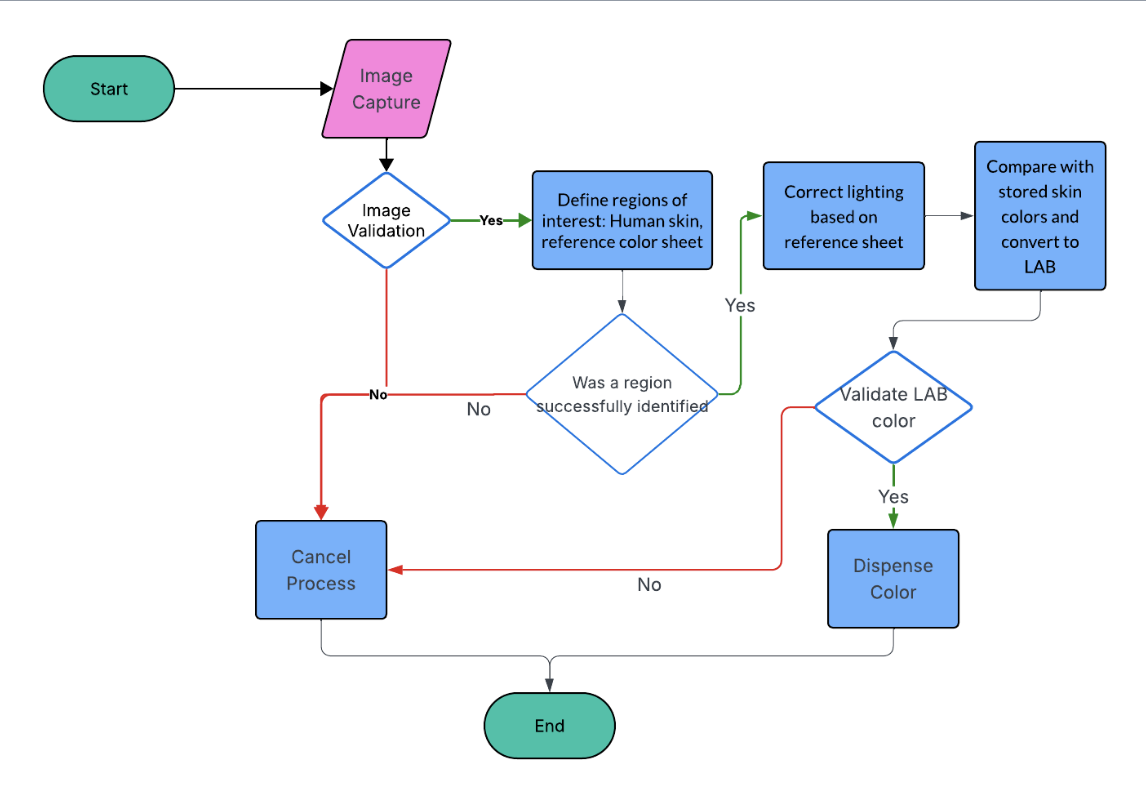
\includegraphics[width=0.8\textwidth]{assets/userflow.png}
        \caption{User Flow Diagram}
    \end{figure}

    \section{Computer Vision Pipeline}

    \section{Color Correction Algorithm}

    \section{Foundation Formulation}

    \section{Raspberry Pi Integration}

    \section{User Interface}

    \section{User Manual}

    %===========================ELECTRICAL ENGINEERING DESIGN===========================

    \chapter{Electrical Systems Design}

    \section{Circuit Schematic and Breadboard Design}

    \section{Signal Conditioning and Safety Considerations}

    %===========================RESULTS===========================

    \chapter{Results and Analysis}

    \section{Testing Protocol}

    \section{Color Accuracy}

    \section{System Performance}

    %===========================DISCUSSION===========================

    \chapter{Discussion}
    
    \section{Limitations}
    
    \section{Future Work}

    %===========================CONCLUSION===========================

    \chapter{Conclusion}

    %===========================REFERENCES===========================
    
    \chapter*{References}

    \addcontentsline{toc}{chapter}{References}

    %===========================SOFTWARE DESIGN===========================

    \appendix

    \chapter{Pseudocode Listings}
    \begin{figure}[H]
        \centering
        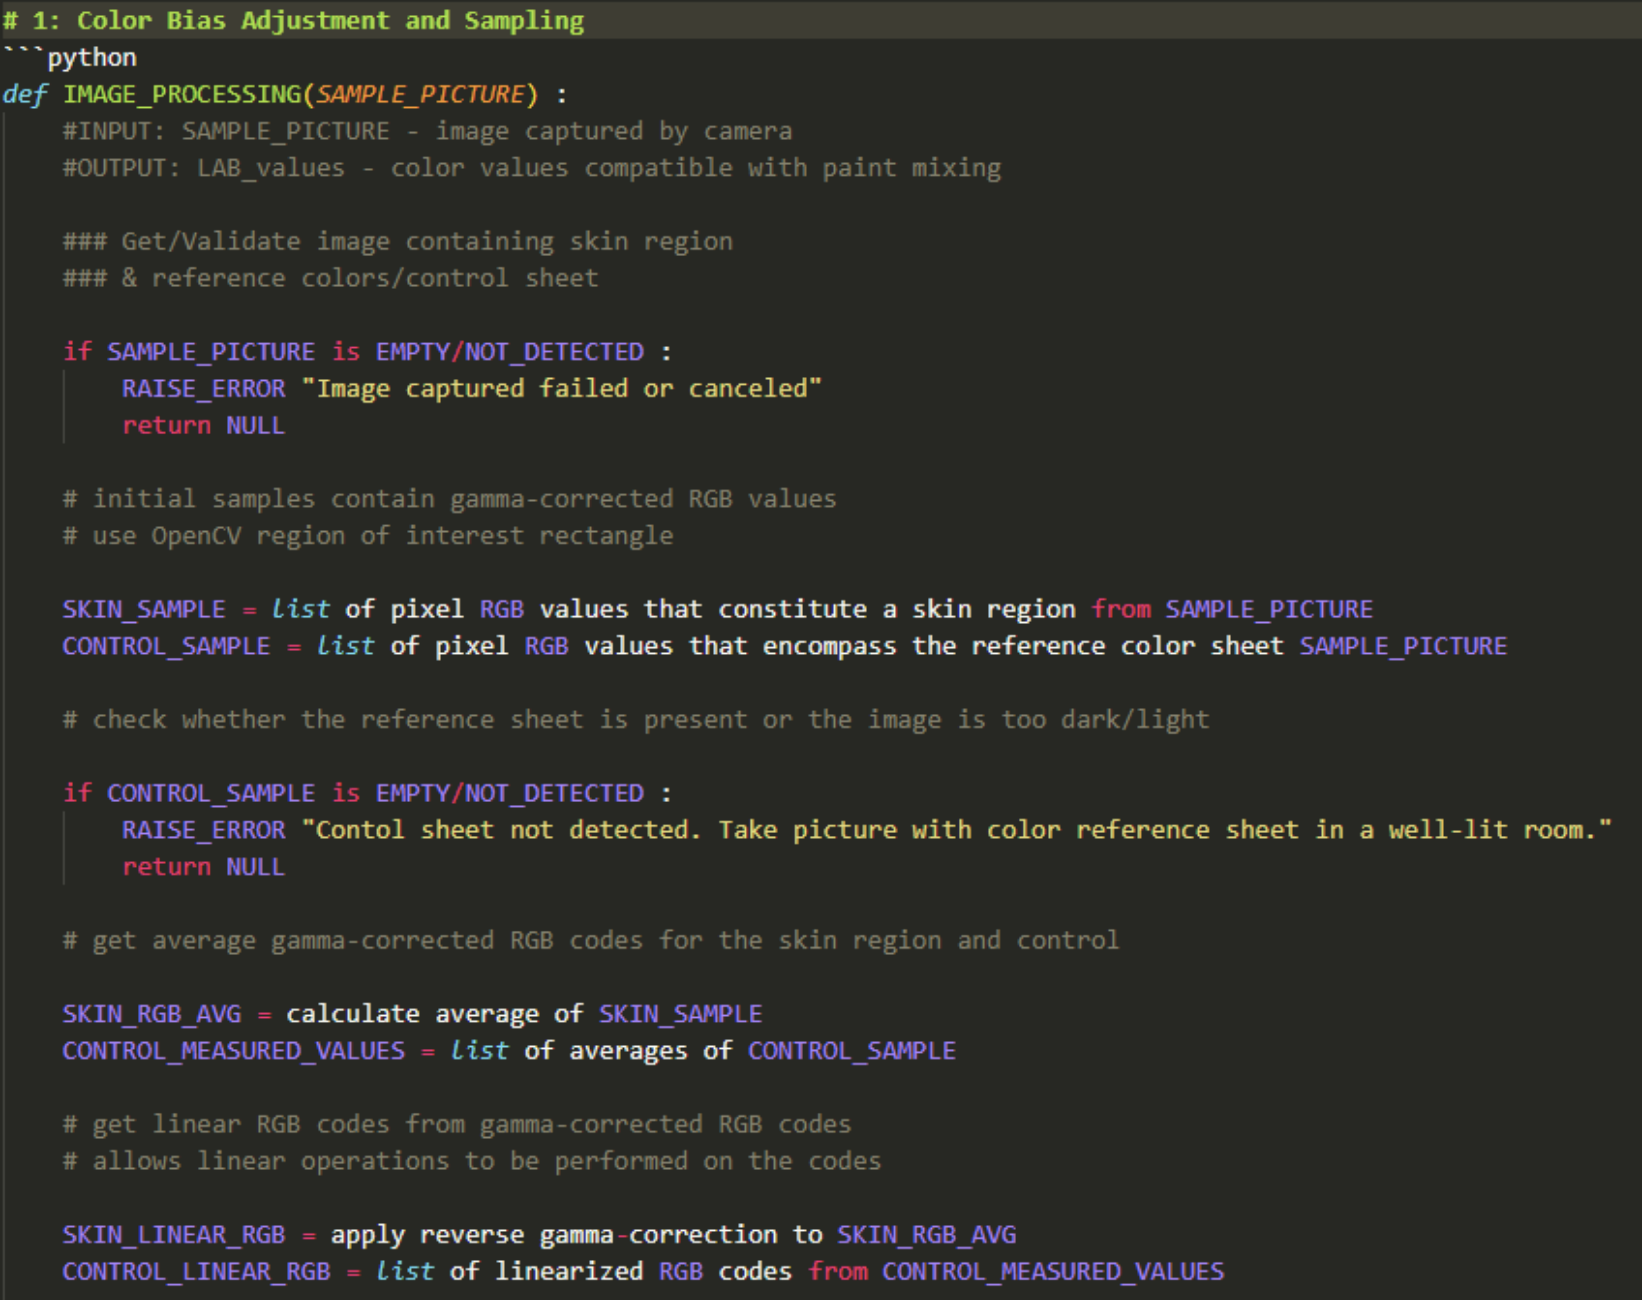
\includegraphics[width=0.8\textwidth]{assets/pseudocode1.png}
        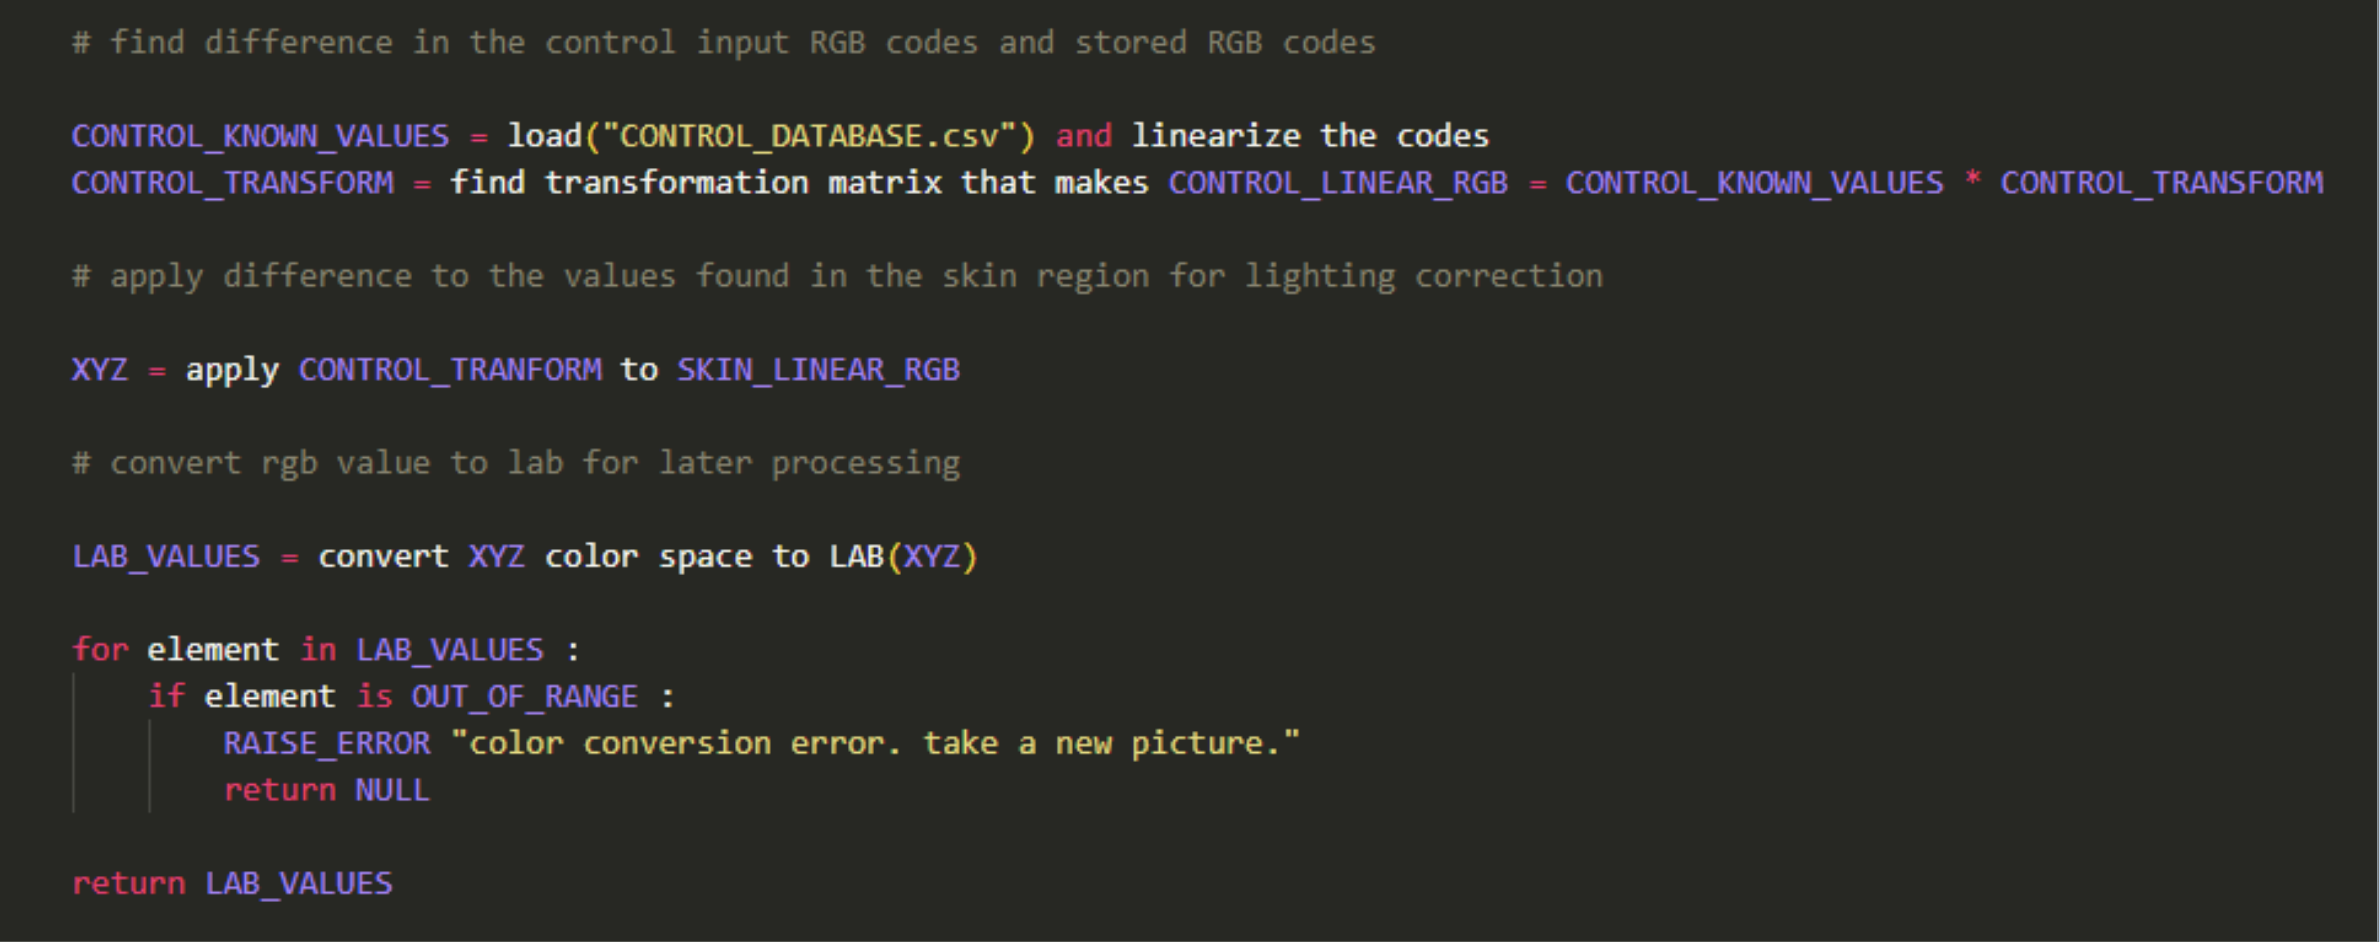
\includegraphics[width=0.8\textwidth]{assets/pseudocode2.png}
        \caption{Pseudocode: Image Processing Algorithms.}
    \end{figure}

    \chapter{Wiring \& Safety}
    \begin{figure}[H]
        \centering
        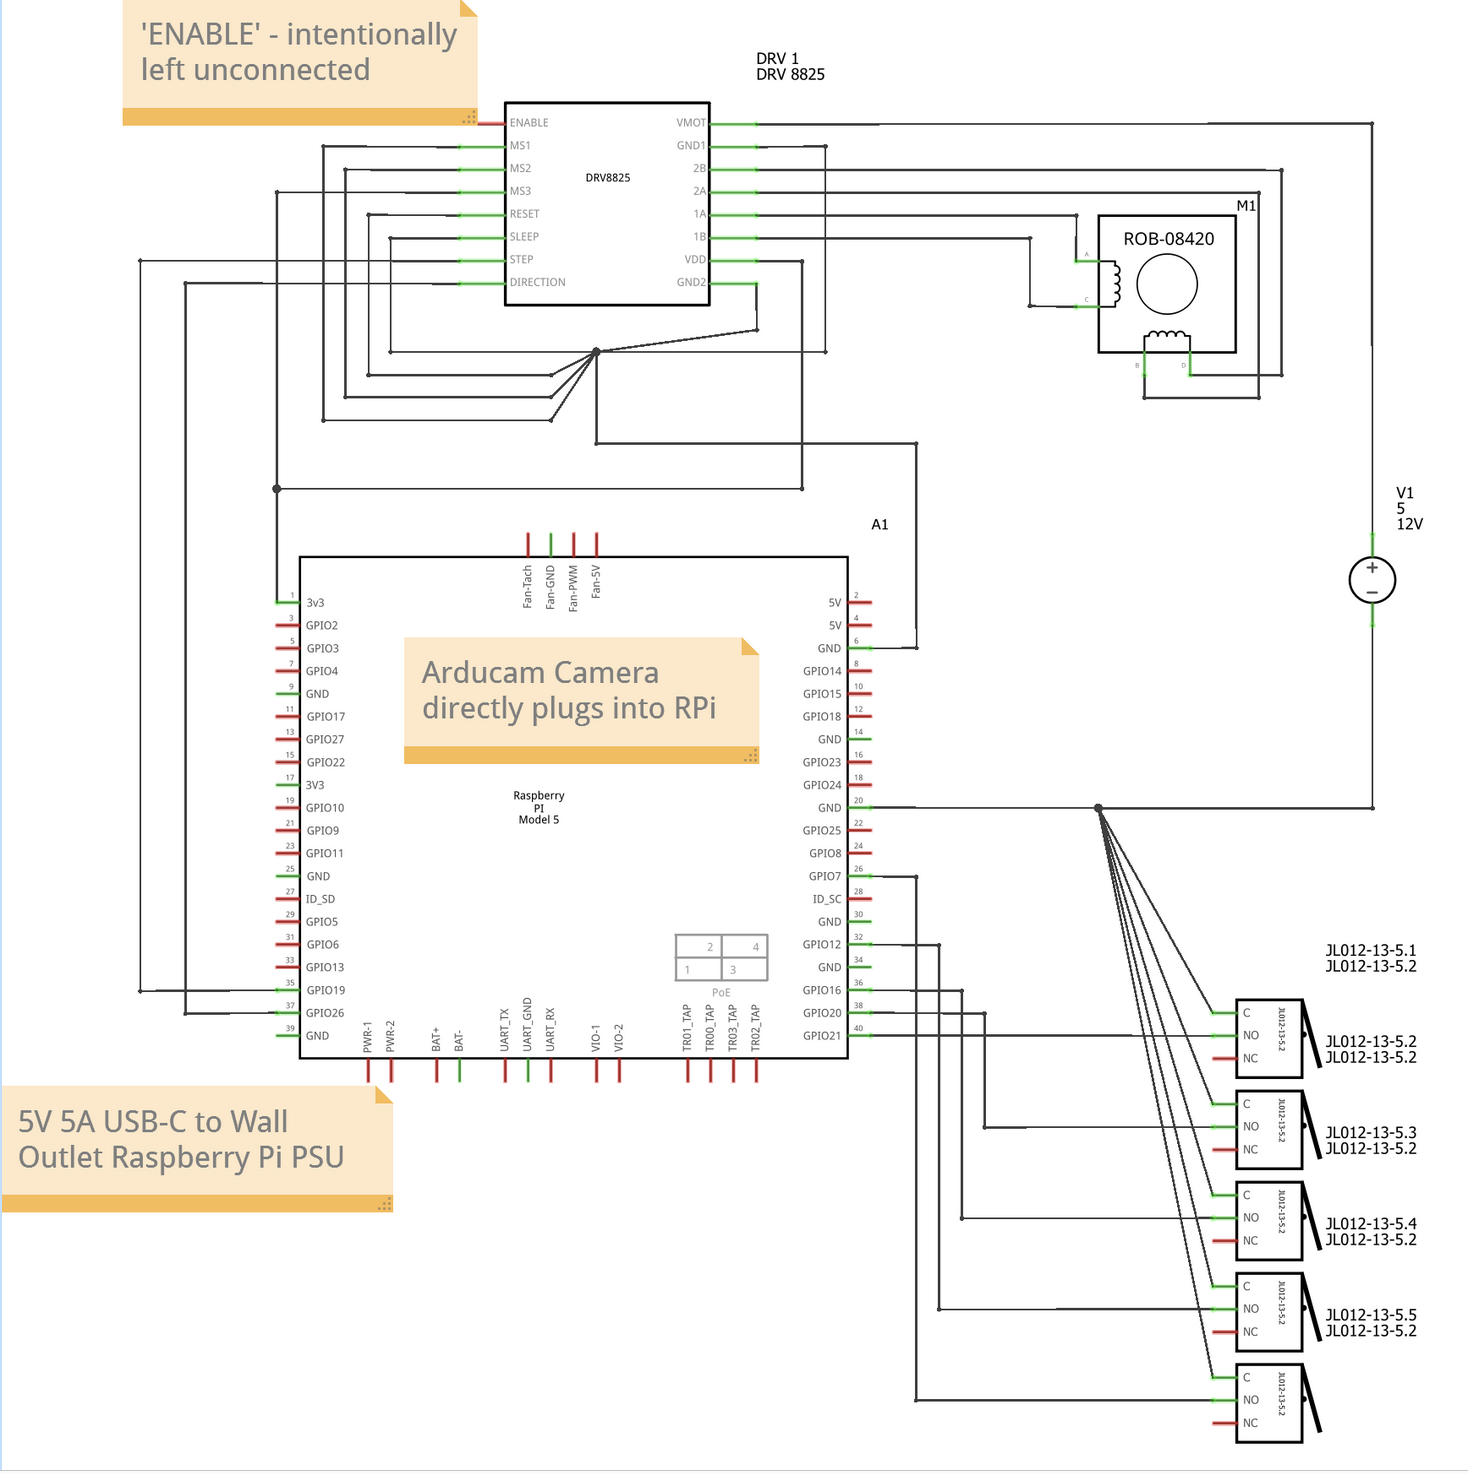
\includegraphics[width=0.8\textwidth]{assets/wiring.png}
        \caption{Wiring Diagram}
    \end{figure}

    \chapter{Data Schemas}


\end{document}
